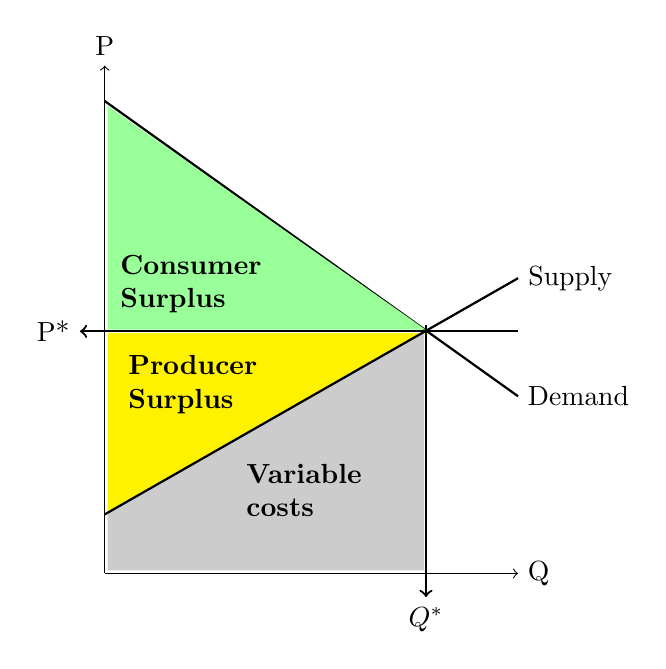
\begin{tikzpicture}[scale=1.5]
%\draw[thick,color=gray,step=.5cm, dashed] (-0.5,-.5) grid (3,3);
\draw[->] (0,0) -- (3.5,0) node[right ] {Q};
\draw[->] (0,0) -- (0,4.3) node [above] {P};
\draw[thick] (0,4) -- (3.5,1.5) ; \node [right]at (3.5, 1.5 ) {Demand}; 

\draw[thick,->] (2.72,2.1) -- (2.72,-.2) node[below] {$Q^*$};
\filldraw [color=green!40]  (0.03,2.07)-- (0.03,3.95)--(2.7,2.07)--cycle;
\filldraw [color=yellow] (0.03,2.03)-- (0.03,.515)--(2.7,2.03)--cycle;
\filldraw [color=gray!40](0.03,.515)--(2.7,2.03)-- (2.7,0.03)--(0.03,0.03)--cycle;
\draw[thick,<-] (-.21,2.05)node[left]{P*}  -- (3.5,2.05) node[above left] {}; 
%\fill[blue, opacity=.25]  (0,4) -- (1.86,2.1) --  (0,2.1) --cycle; 
%\fill[green] (0,.52) -- (1.82,2.1) --  (0,2.1) --cycle; 
\draw[thick] (0,.5) -- (3.5,2.5) node[right] {Supply};
\path (.7,2.45) node [text width=1.7cm](labelRent) {\textbf{Consumer\\Surplus}};
\path (.7,1.6) node [text width=1.5cm](labelRent) {\textbf{Producer\\Surplus}};
\path (1.7,.7) node [text width=1.5cm](labelvarcost){\textbf{Variable\\costs}};
%\path (1.7,-1) node [black](labePC) {With producible capital};
\end{tikzpicture} 
% \path (.7,2.45) node [text width=1.7cm](labelRent) {\textbf{Consumer\\ Surplus}};
% \path (.7,1.6) node [text width=1.5cm](labelRent) {\textbf{Producer\\ Surplus}};
% \path (1.7,.7) node [text width=1.5cm](labelvarcost){\textbf{Variable\\ costs}};